\documentclass[conference]{IEEEtran}

\usepackage{hyperref}
\usepackage{graphicx}\graphicspath{ {images/} }
\usepackage{listings}
\usepackage{flushend}
\usepackage[section]{placeins}
\usepackage{amssymb}
\usepackage{lipsum}

% Hyphenation correction
\hyphenation{op-tical net-works semi-conduc-tor}

\makeatletter
\AtBeginDocument{%
  \expandafter\renewcommand\expandafter\subsection\expandafter{%
    \expandafter\@fb@secFB\subsection
  }%
}
\makeatother

\begin{document}

\title{Text Mining the IEEE Xplore Database}
\author{\IEEEauthorblockN{Stuart Miller}
\IEEEauthorblockA{Department of Electrical and\\Computer Engineering\\
Missouri University of Science \& Technology\\
Rolla, Missouri 65409\\
Email: \href{mailto:sm67c@mst.edu}{sm67c@mst.edu}\\
Web: \url{http://web.mst.edu/\textasciitilde sm67c}}
}

\maketitle

\begin{flushright}\end{flushright}
\begin{abstract}
Keeping up with the current state of the academic world involves staying knowledgeable about current trends in academic literature; but, with thousands of papers published each month this can be an insurmountable task. The use of natural language processing (NLP) techniques can be applied as an aid to this task and can even go so far as to provide unique insights about the current state of a field of study as a whole. By applying latent Dirichlet analysis and other NLP tools to currently published works, a researcher can gain knowledge about the field, analyze current trends, and assess the fitness of their own work.
\end{abstract}

\section{Introduction}

A significant part of any researcher's time is dedicated to maintaining an involvement in current publications in one's field. Any researcher must spend time parsing the current state of the field and targeting relevant papers in order to obtain the latest trends, proposals, and ideology. This is particularly true for computation based fields.

One of the preeminent publishers in the Electrical and Computing field is the Institute of Electrical and Electronics Engineers (IEEE). IEEE maintains an online database of all presence and past publications in digital form. Containing 176 different regular publications and countless more event proceedings, keeping fully up to date with the state of any field encompassed by the IEEE proves to be a momentous task.

Therefore, an investigation into the applicability of text mining and natural language processing (NLP) is presented. The goal is to provide a tool that can be useful for researchers to evaluate the current state of their field and to be able to profile both current preeminent papers as well as their own published (or pre-published) work.

\section{Background}

\subsection{Term Frequency-Inverse Document Frequency}

Proposed in 1972 as part of work done at the Cambridge Computing Laboratory, the term frequency-inverse document freuency (TF-IDF) algorithm \cite{sparck1972statistical} provides a quick and easy way to rank a document's relevance to a particular term. Initially proposed by Jones, the TF-IDF is a valuable concept for ranking within bodies of literature. In short, the TF-IDF ranking for a particular term in a particular document is comprised of the product of the term frequency and the inverse document frequency (\ref{eq:tfidf}).

Term frequency is defined as the number of times term $t$ appears in document $d$ over the total number of terms in the document (\ref{eq:tf}). Inverse document frequency is defined as the log of the inverse of the total number of documents containing term $t$ (\ref{eq:idf}).  Various weightings and smoothings can further be applied to fine-tune a result for a a particular data set if so desired. Weightings can be binary, log-based, or scaled by any custom factor.

\begin{equation}
\label{eq:tfidf}
tfidf = tf(t,d) \cdot idf(t,d)
\end{equation}

\begin{equation}
\label{eq:tf}
tf = \frac{t \in d}{\forall t \in d}
\end{equation}

\begin{equation}
\label{eq:idf}
idf = \log \Big( \frac{D}{d \in D : t \in d} \Big)
\end{equation}

Although the inner working of Internet search engines are a closely guarded corporate secret, it is theorized that the basis of each is a variation of a TF-IDF ranked search, a notion investigated and exploited by Lin and Chi in \cite{6845978}.

Unfortunately, the TF-IDF algorithm is restricted to providing a rather narrow view. By itself, it is incapable of providing insights regarding broad trends across an entire document sets as it's domain is restricted to scoring against a single term at a time. Nonetheless, work on the TF-IDF algorithm is indeed ongoing. Research such as that brought forth by Yang and Guo proposes a new variation and weighting scheme for big data applications \cite{7560393}, a topic that is ever relevant to modern day technology. In fact Yang and Guo even go so far as to propose a novel new parameter to the TF-IDF that adjusts the ranking based on the ranking of nearby terms.

\subsection{Latent Dirichlet Allocation}

By applying to Bayesian inference to developing probability simplexes, the latent Dirichlet allocation (LDA) algorithm was born. It was developed independently by Blei\cite{blei2003latent} and Pritchard\cite{pritchard2000inference}. The LDA aims to produce a "distribution of distributions", by providing a distribution of topic probabilities for each document. That is, each of a document's terms must be fitted to topics and each topic must be fitted to documents.

The result is a distribution of indexed topics to each document. Topics are referenced only by index number and therefore are not necessarily semantically defined. Thus, an important step of using the results from a LDA fitting is to classify resulting topics and relate them to real-world concepts.

\begin{figure}
	\centering
	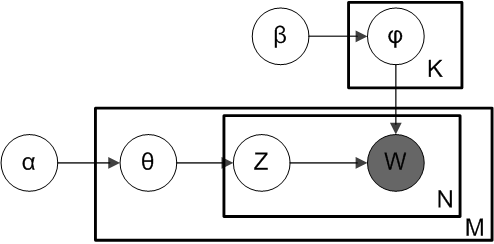
\includegraphics[width=2.5in]{lda_plate_model.png}
	\caption{LDA Plate Model, graphic from Blei \cite{blei2003latent}}
	\label{fig:lda_plate_model}
\end{figure}

To do this, the LDA initializes random topic mixtures across each document. The variables $\alpha$ and $\beta$ represent the starting Dirichlet distribution parameters for assigning the per-document topic distribution and the per-topic word distribution, respectively. These parameters are the defining variables of the LDA and represent the probability distribution across that comparison. If the Dirichlet parameter is equal to one, it represents an even distribution; higher represents a distribution concentrated in the middle of both variables, lower represents concentrated on the edges near to the bounds of the variables. As the goal here is to obtain the primary topic(s) of each document and word, uneven distributions are highly desirable. In figure \ref{fig:lda_plate_model}, the plate model is shown. Here, the initial Dirichlet parameter $\alpha$ is assigned to the topic distributions per document ($\theta_1 ... \theta_M$  are $K$-dimensional vectors containing the Dirichlet parameter for each of $M$ documents) and the initial Dirichlet parameter $\beta$ is assigned to the word distribution per topic ($\phi_1 ... \phi_K$  are $W$-dimensional vectors containing the Dirichlet parameter for each of $W$ total words). The innermost plate shows the results, $Z_{mn}$, which represent the topic for the $n$th word in document $m$. More generally, $W_{mn}$ is the entire body's collection of words assigned to topics. The words associations can then be summed back across the original documents in which they appear, each word's own topic association adding into an overall topic association for the document as a whole.

\begin{equation}
\label{eq:gibbs_samp}
p(z_d = k) \propto \frac{\alpha_t\beta}{\beta W + K} + \frac{K_{d}\beta}{\beta W + K} + \frac{(\alpha_t + W_{k})}{\beta V + K}
\end{equation}
	
In order to tune the Dirichlet parameters, the collapsed Gibbs sampling method of Bayesian learning is used. Outlined by Yao, et. al.\cite{yao2009efficient}, collapsed Gibbs sampling is the commonly accepted variation for NLP, as it takes advantage of the sparsity of vocabulary. That is, not all words will appear in all documents. Collapsed Gibbs sampling takes the assumption of the given Dirichlet parameters and evaluates it's likelihood by applying to the current body of documents. The base method involves sampling the probabilities $p(A|B,C)$, $p(B|A,C)$, and $p(C|A,B)$. For the LDA, this would involve sampling the choice of topic vs all other words' topics, the choice of topic vs all topics in the document, the choice of topics vs other words not in the document, the choice of topic vs other words in the topic and their documents, and so on.  In order to "collapse" the sampling, the probability that a particular word $Z$ in document $d$ is assigned to topic $k$ can be represented by a proportion of three terms (\ref{eq:gibbs_samp}). It is a summation of the the current parameters assigned, the parameters of the other topics in this document $K_d$, and the parameters assigned other words that are assigned to this topic $W_k$ across the entire body. Such a method cuts out summing every combination of parameters and focuses on the parameters combinations most influential to determining a valid probability.

As it is a type of structured learning, LDA does require significantly more computation time and this serves as it's main drawback; but, it provides much more comprehensive data. As such, the presentation here will utilize the LDA model as the basis for most of its analysis.

LDA is widely studied in the current academic body of work. Countless investigations into its application for modern-day technologies are begin shown. For example, Diop, et. al. \cite{8323808} present an application of LDA for use in modern video surveillance. In place of words, they use motion information, instead of topics they use defined events, and instead of documents they use camera views. This just goes to show the relevance of the LDA algorithm in the current state of the field.

\subsection{Latent Semantic Analysis}

Patented in 1988, the latent semantic analysis (LSA) algorithm \cite{patent4839853}, relies on singular-value decomposition of a term-document matrix. As opposed to the TF-IDF which produced a single term ranking, or LDA which produced a probability distribution, the LSA produces a $k$-dimensional topic vector (where $k$ represents the number of topics chosen).

Computationally, the LSA starts with a term-document matrix of $m$ terms by $n$ documents. The term-document matrix undergoes singular value decomposition $M = U \Sigma V^*$ where $U$ is an $m*m$ unitary matrix over $\mathbb{R}$, $V$ is an $n*n$  unitary matrix over $\mathbb{R}$, and $\Sigma$ is a diagonal $m*n$ matrix containing the singular values of $M$. Take the resulting matrix and zero out all but the top $k$ term rows, where $k$ is the desired number of topics. The remaining matrix represents $n$ $k$-dimensional topic vectors.

LSA does rely on some heavy matrix-math computations, but is at its heart only using matrix math; no learning algorithms. Accordingly this means its runtime consistently falls in between that of LDA and TF-IDF.

Due to the inherent complexity of parsing highly dimensional data, the results of the LSA were deemed not worth the time to interpret for the average researcher for the purposes of this project. As the goal is to provide a solution that is accessible and easily viewable, LSA doesn't produce results that are as easily parsed by the target audience.

\section{Summary and Specifications}

The goal herein is to provide a research aid to assist those who wish to analyze the current state of an academic field and assess the preeminent literature available. As mentioned in the introduction, this presentation focuses merely on papers found in the IEEE XPlore database. Access to the API is available upon request at \url{https://developer.ieee.org/}.

The endeavor presented below will perform a number of analyses on the obtained data, but focus primarily on the LDA algorithm as described about. The computing environment used will be MATLAB, as the goal is to provide an easy-to-use tool and most researchers obtain at least a modest amount of familiarity with MATLAB at some point in the career. MATLAB's built-in latent dirichlet allocation function will be used. This function works off of collapsed Gibbs sampling and has been optimized for the environment. This provides a significant runtime advantage as opposed to making use of a custom or third-party LDA algorithm not ingrained in the MATLAB environment.

In order to parse the contents of the paper efficiently, only the abstracts will be taken into account. By design, the abstract is to be a brief but informative synopsis of the proposition being made in the paper. Most papers average around 200 word for the abstract, making for a good size for processing (about 1MB of uncompressed data per 1000 papers).

\begin{figure}
	\centering
	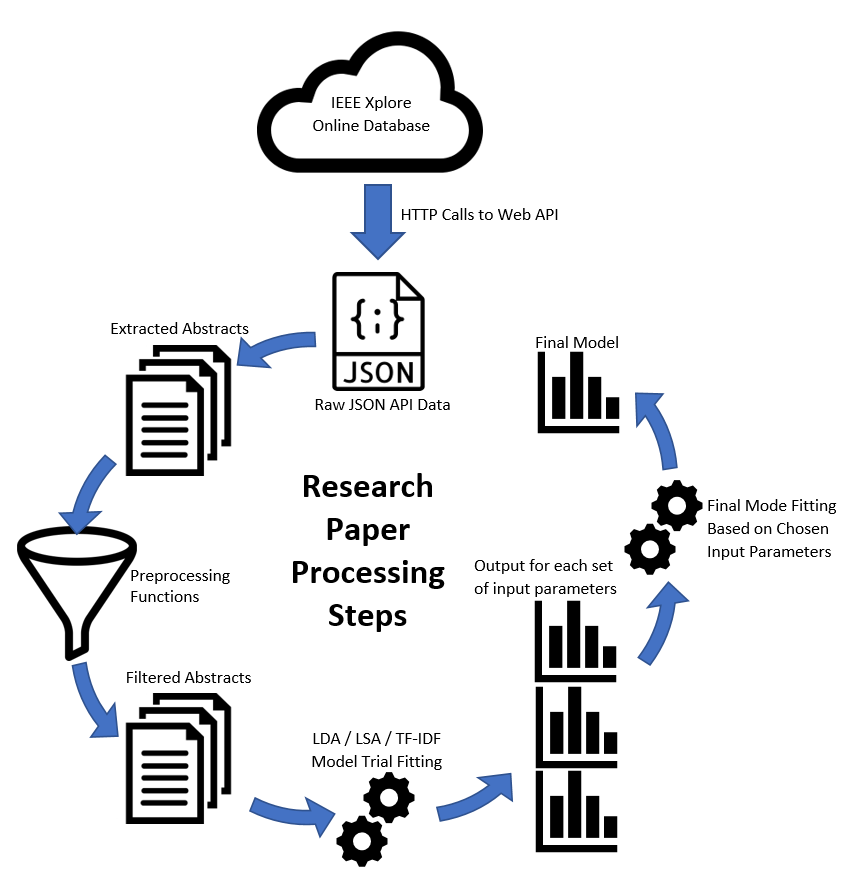
\includegraphics[width=3.4in]{flowchart.png}
	\caption{Document Processing Flowchart}
	\label{fig:flowchart}
\end{figure}

Each paper's metadata was downloaded via automated HTTP get requests to the IEEE API. Upon being downloaded, each paper's abstract and contextual data were extracted and the remaining excess discarded.

In order to further reduce the computation required to parse text in each paper's abstract, several preprocessing steps were taken. All punctuation, numerals, control characters, and other extraneous symbols were removed and all characters are normalized to lowercase forms. Subsequently, each paper was fed through a Porter stemmer. Formalized by Porter in 1980 \cite{porter1980algorithm}, the Porter stemming algorithm normalizes prefixes and suffixes to common English words. (For example: "estimated", "estimator", and "estimation" would all be normalized to "estimat".) Common stopwords such as "a, "the", "that", etc. were also removed from the abstract. Finally the abstract was reduced to a list of stemmed words and their frequency counts, commonly known as the "bag of words" model. 

After processed data had been obtained, trial model fitting occurred. Both the LDA and LSA algorithms require s specified number of topics to be chosen beforehand. To facilitate this, several test fits were run for various topic sizes. Additionally, other parameters such as variations of the preprocessing steps can take place here to ensure the the final model is acceptable. Once models have been produced, it is vital the models are both mathematically viable and human-readable. Topics may be mathematically sound, but must be categorically relevant to a human interpreter or the model isn't worth anything to a potential researcher. Once parameters have been fine-tuned and a final number of topics has been chosen, the final model fitting can be run and the data can be stored for later analysis. For this presentation, the LDA models generally proved to be the most balanced and provided graphical output that was easily interpreted.

This overall flow is visualized in figure \ref{fig:flowchart}.

\section{Detailed Design: Breakdown of Papers from 2018}

\begin{figure}
	\centering
	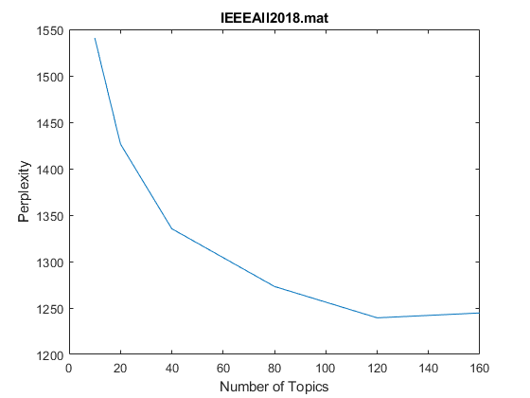
\includegraphics[width=3.4in]{all2018_ppl_120.png}
	\caption{Perplexity of various topic counts for the All2018 data set}
	\label{fig:all2018_ppl_120}
\end{figure}

\begin{figure*}[tb]
	\centering
	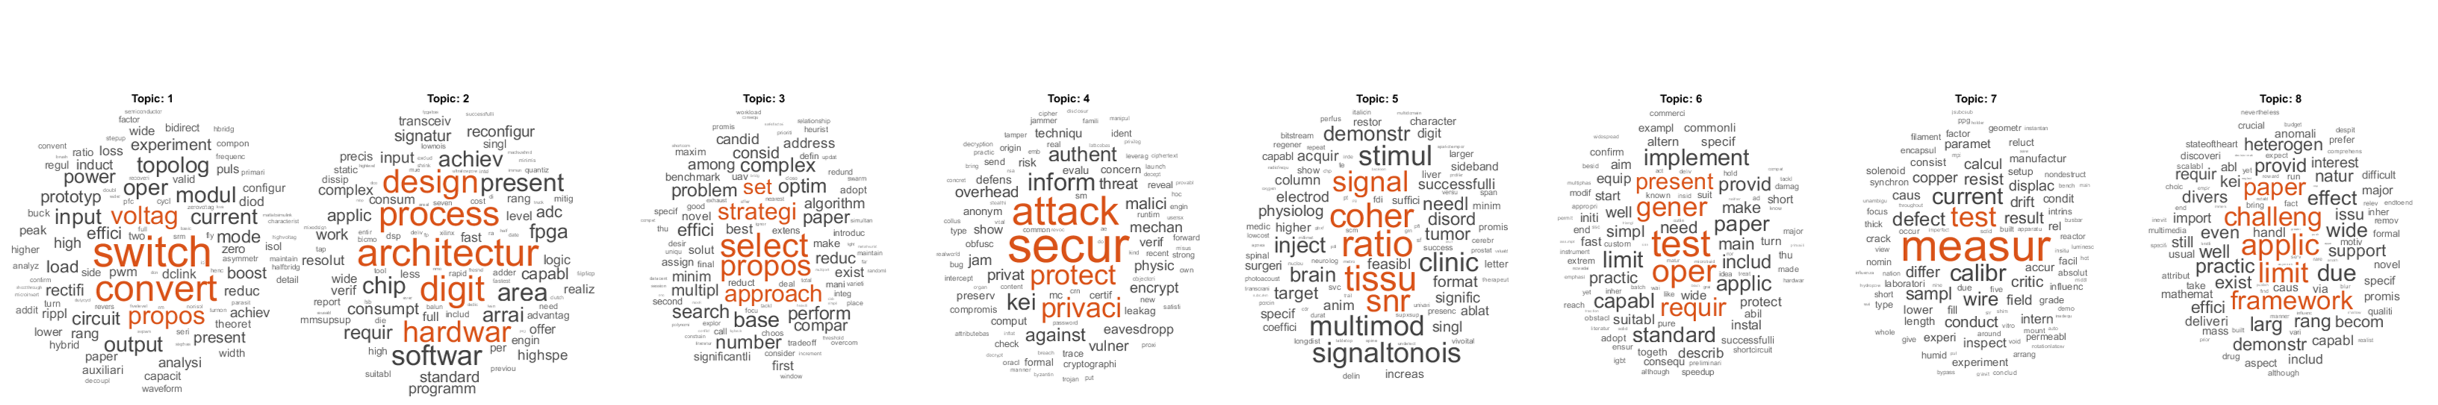
\includegraphics[width=7.0in]{all2018_cloud_120.png}
	\caption{Word clouds for the first 8 topics of the All2018 data set, fit with 120 topics}
	\label{fig:all2018_cloud_120}
	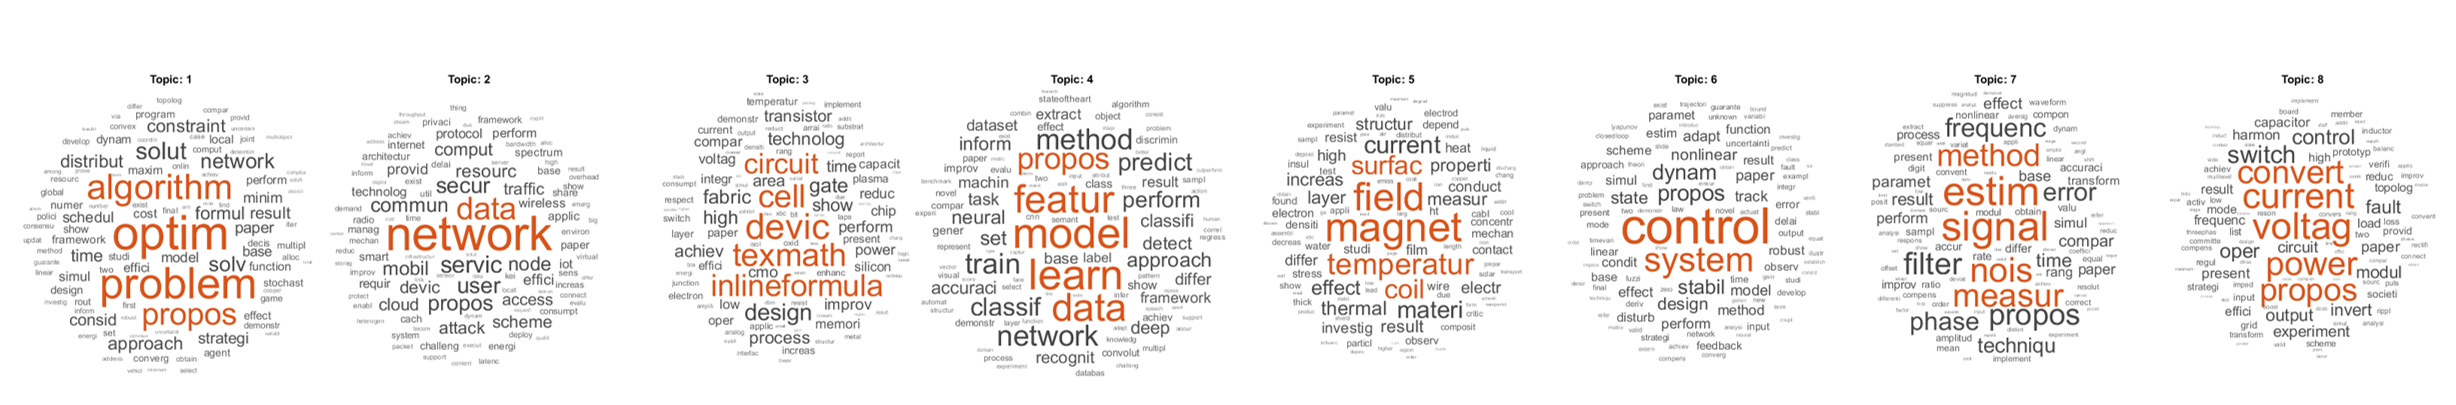
\includegraphics[width=7.0in]{all2018_cloud_20.png}
	\caption{Word clouds for the first 8 topics of the All2018 data set, fit with 20 topics}
	\label{fig:all2018_cloud_20}
\end{figure*}

\begin{figure}
	\centering
	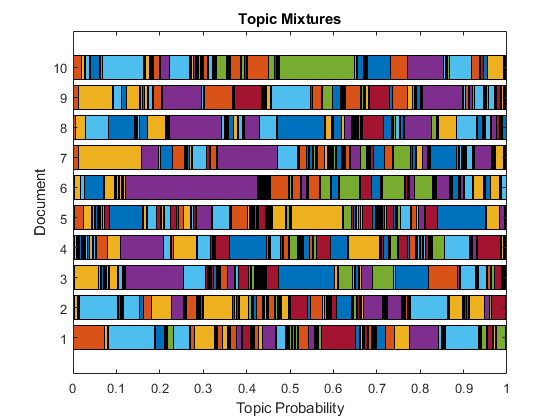
\includegraphics[width=3.4in]{all2018_lda_120.png}
	\caption{Topic mixtures for the first 10 papers of the All2018 data set, fit with 120 topics}
	\label{fig:all2018_lda_120}
\end{figure}

\begin{figure}
	\centering
	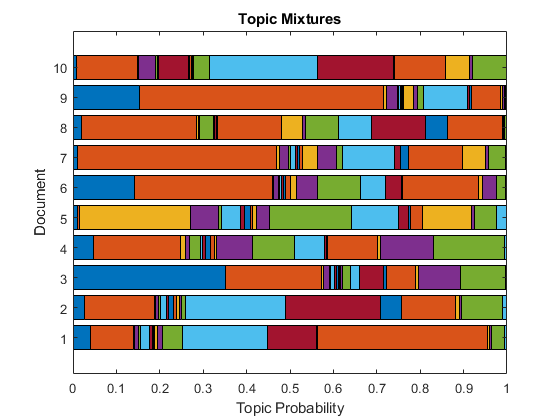
\includegraphics[width=3.4in]{all2018_lda_20.png}
	\caption{Topic mixtures for the first 10 papers of the All2018 data set, fit with 120 topics}
	\label{fig:all2018_lda_20}
\end{figure}

To get an initial view of the field and to prove the effectiveness of various algorithmic approaches, the first data set considered is a collection of all papers currently published (or accessible as an early access copy of a publication) in calendar year 2018. This data set was pulled from the IEEE API in mid March 2018, and comprised approximately 11 weeks worth of publications, containing 21,985 papers.

Running an LDA against a subset of the papers to determine a fit resulting in the perplexity graph shown in figure \ref{fig:all2018_ppl_120}. Extrapolating from the trial fits suggests that 120 may be an optimal number of topics to select. The resulting topic distribution for the first 10 documents can be seen in figure \ref{fig:all2018_lda_120}. Unfortunately, these are not very clean topic designations. For most documents, it is near impossible to point to any one topic with a significant plurality. Examining word clouds (figure \ref{fig:all2018_cloud_120}) for the topics again reiterates the point that these topics are far too ambiguous to be useful. Even though the mathematics points to a large topic count like 120 as providing the best fitting model, it is useless if the results can't be easily parsed by a human. Keeping in mind that the primary goal of this proposal is to provide a model to aid the human researcher, the number of topics must be reduced.

At this point the topic count may be adjusted by the researcher depending on what their needs are. If gaining an overall view of broad fields is the intended goal, it would be desirable to pick a very small topic count, but if there is an interest in the ability to drill down into specific sub-fields, a slightly large topic count could be beneficial. Knowing that the all2018 data set contains papers from all across electrical and computer engineering, 20 topics will be chosen to create broad categories and serve as a proof of concept. Re-running the LDA and plotting the topic distribution reveals the distribution shown in figure \ref{fig:all2018_lda_20}. It is now evident that papers feature much more prominently in distinct categories.

This distinction can be further observed when examining the topic contents. The first 8 topics for both fits have been grouped into word clouds (figures \ref{fig:all2018_cloud_120} and \ref{fig:all2018_cloud_20}), a format in which the size of each word is directly proportional to it's frequency within (and relevance to) that topic. Notice that topics 6 and 7 in the 120 topics fitting are very similar and many don't have any bearing on any one particular field of study. On the other hand, nearly every topic features clear and concise keywords for a field. An interesting sidenote is that topic 3 in the 20-topic fitting aggregated some TeX keywords, encompassing papers that used inline math mode within their abstracts.

\begin{figure}
	\centering
	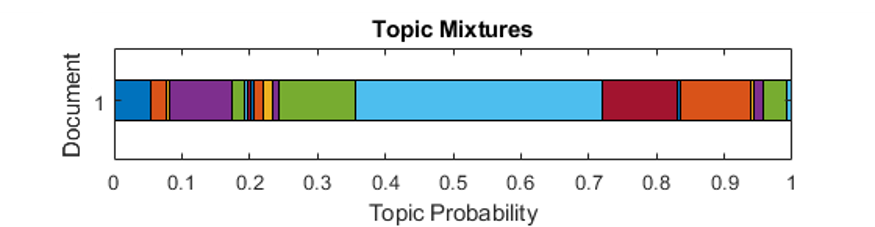
\includegraphics[width=3.0in]{wunschpaper_topics.png}
	\caption{Topic Distribution for "Survey of Clustering Algorithms" \cite{1427769}}
	\label{fig:wunschpaper_topics}
\end{figure}

\begin{figure}
	\centering
	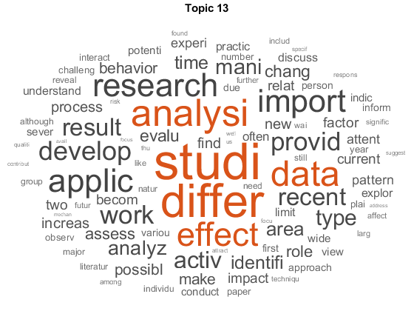
\includegraphics[width=3.4in]{wunschpaper_wordcloud.png}
	\caption{Word cloud for primary topic of "Survey of Clustering Algorithms" \cite{1427769}}
	\label{fig:wunschpaper_wordcloud}
\end{figure}

\subsection{Model Applicability}

Assuming that this model is accurate, it should be possible to apply it to any given research paper to fit for topic proportions. Take, for example, Wunsch and Xu's "Survey of Clustering Algorithms". Applying the established LDA model to this paper yields a clear plurality for topic 13. As this is a survey paper, one would expect its abstract to be broad and to touch on multiple different sub-disciplines of computational intelligence and clustering. Appropriately, the defining words of topic 13 suggest comparative analysis with key word stems such as "analysi/analyz", "differ", "studi", etc.

In such a way, a research could evaluate the fitness of their own paper against the current trends to see if it is a good fit for their target subject. Such a tool could prove very useful pre-publication.

\subsection{TF-IDF Analysis}

\begin{figure}
	\centering
	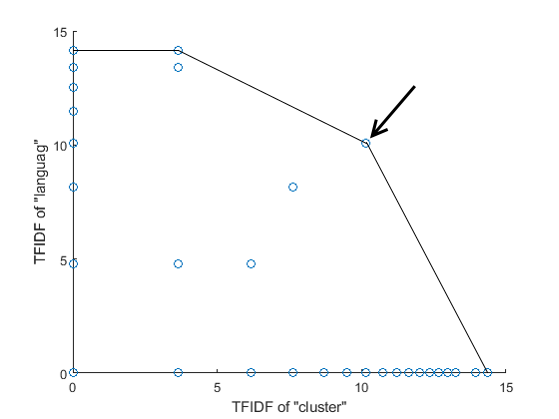
\includegraphics[width=3.4in]{tfidf-pareto.png}
	\caption{Documents ranked by TF-IDF of "cluster" and "language" with highlighted Pareto front}
	\label{fig:tfidf_pareto}
\end{figure}

The results can be further examined by a more in-depth TF-IDF analysis. A TF-IDF ranking can be obtained by selecting keyword(s) to index off of. In this instance, take the self-referential terms "language" (stemmed to "languag") and "cluser". Ranking and sorting the entire body results in several papers that score well in each. Plotting both on a single X-Y plane and analyzing yields a Pareto front containing several papers \ref{fig:tfidf_pareto}. The indicated point on the center-most part of the front belongs to paper 7568, Iwata Hirao and Ueda's "Topic Models for Unsupervised Cluster Matching," a paper that presents a model for clustering both English and German documents based on their linguistic similarities \cite{8125189}.

This is undoubtedly an apt match for the topic. In face, this can be confirmed by performing a web search on IEEE's website for the same terms. As of April 2018, Iwata, Hirao, and Ueda's paper appears on the first page of search results alongside several similar papers that were published outside of the time frame of the IEEEAll2018 data set. As an aside, this speaks to the significance of the TF-IDF algorithm and this similarity likely indicates that IEEE's own internal document search engine may utilize a variation of TF-IDF in it's ranking.

\section{Experimental Results: Articles from Selected Publications}

In order to drill down deeper and provide a more fine-grained and compartive analysis, additional data sets were retrieved from the IEEE Xplore API. Each data subset contained all the published articles for a particular publication. Once again, LCD topic models were ran on a training partition of each and plotted. Figures show perplexity for each model fitting broken down by type of article: journals, transactional publications, and conference and workshop proceedings respectively.

\begin{figure}
	\centering
	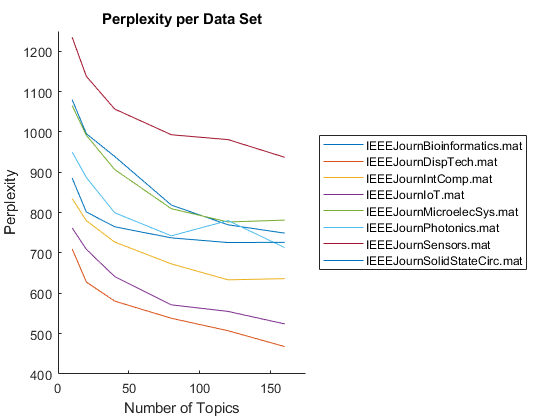
\includegraphics[width=3.4in]{journ_ppl.png}
	\caption{Perplexity for Papers in Various Journals}
	\label{fig:journ_ppl}
\end{figure}

\begin{figure}
	\centering
	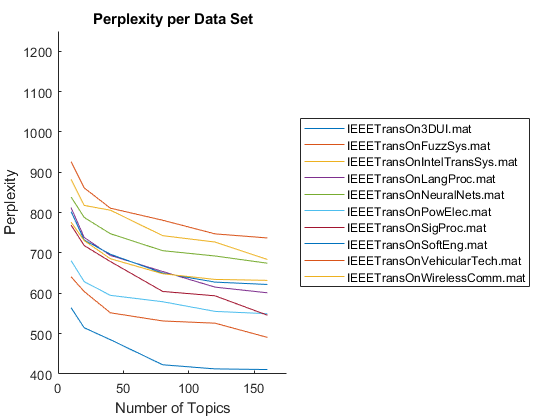
\includegraphics[width=3.4in]{trans_ppl.png}
	\caption{Perplexity for Papers in Various Transactional Publications}
	\label{fig:trans_ppl}
\end{figure}

\begin{figure}
	\centering
	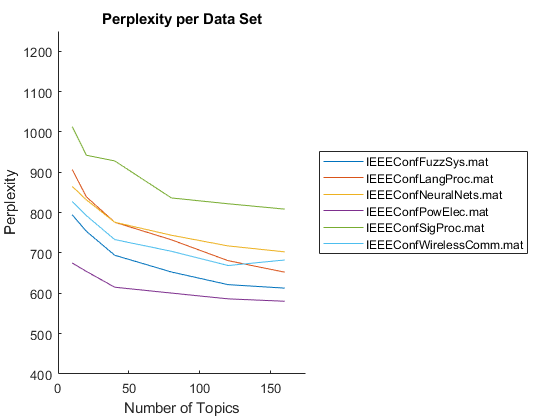
\includegraphics[width=3.4in]{conf_ppl.png}
	\caption{Perplexity for Papers in Various Conference Proceedings}
	\label{fig:conf_ppl}
\end{figure}

\begin{figure}
	\centering
	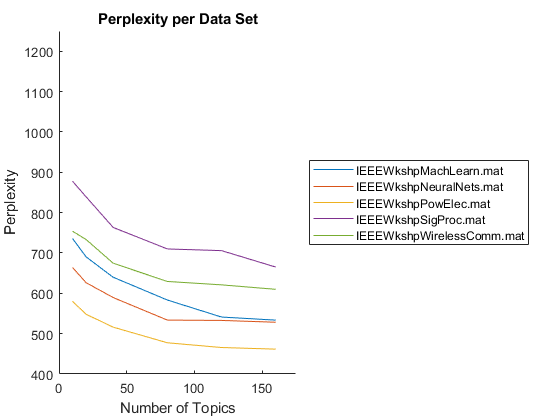
\includegraphics[width=3.4in]{wkshp_ppl.png}
	\caption{Perplexity for Papers in Various Workshop Proceedings}
	\label{fig:wkshp_ppl}
\end{figure}

Note that the journal subsets tend to have a slightly higher perplexity overall. This may be an indication that the topics covered in journal articles are more in-depth and are more dissimilar than other types of publications. While there are distinctions between each type of publication, there is far more variation within each based on subject matter. A potential researcher can draw the conclusion that when concerned with finding the most apt medium to publish their work, the type of publication is not quite as important as the subject matter of the publication. 

Moving forward, the 20-topic model will once again be chosen for each subset. Each perplexity graph shows a sharp decline around 20, but only modest declines after that (particularly so for the conference and workshop subsets), indicating that the 20-topic model is once again a good balance of mathematically viable and human-decipherable.

\begin{figure}
	\centering
	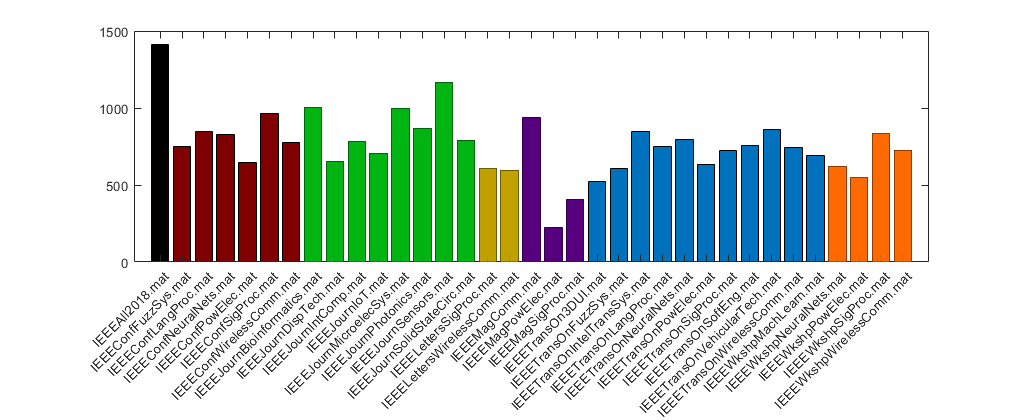
\includegraphics[width=3.8in]{all_ppl.png}
	\caption{Perplexity vs Number of Papers (Documents) per Publication}
	\label{fig:all_ppl}
\end{figure}

When examining this many different data subsets, it is important to weigh the influence of data set size. Smaller data sets may be inherently be more or less complex and therefore come up with more or less comprehensive models accordingly. The perplexity by publication chart (figure \ref{fig:all_ppl}) shows the diversity here. Notice that the IEEE Letters and IEEE Magazines score some of the best fitting models. However, each set included only a few hundred individual articles, wheres most of the journals and transcational publication contained upwards or 10,000 or even 20,000 articles. Logically, it follows that smaller bodies of work are going to contain fewer outliers and thus not push the boundaries of the fit as much. Therefore these results must be interpreted carefully. Figure \ref{fig:size_vs_ppl} plots the relationship between perplexity and quantity of papers in the publication. The relationship can loosely be summed up as number of papers is directly proportional to perplexity. There are a few outliers though, most notably the Conference Proceedings on Power Electronics; it had the second highest number of papers and below average perplexity.

\begin{figure}
	\centering
	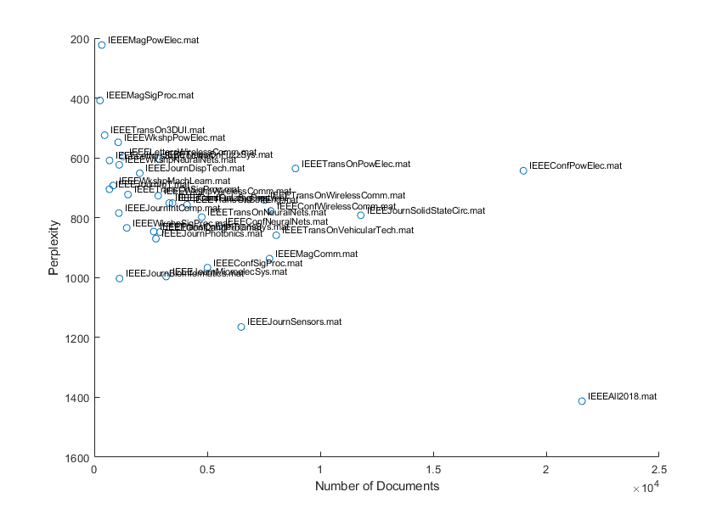
\includegraphics[width=3.4in]{size_vs_ppl.png}
	\caption{Perplexity vs Number of Papers (Documents) per Publication}
	\label{fig:size_vs_ppl}
\end{figure}

One of the primary uses of this analysis tool is to provide a survey of the current state of the art in any particular field. Figure \ref{fig:wirelesscomm_topics} shows word clouds for the topic representations for the Transactions in Wireless Communications. Several key research areas are highlighted. MIMO, or multiple-input, multiple-output antennas, are the subject of much research in the field and as such, topic 7 is entirely devoted to it, containing keywords such as "systems" with different "numbers" of "antennas" featuring "mimo." More current concepts such as channel interference, modulation schemes, protocols to optimize throughput, network security, and much more all receive topics of their own.

A prospective researcher could gain much insight into the the current trends in their field by an analysis such as this. They could even go so far as to fit their own pre-published paper to a topic model in the hopes of satisfying a particular topic, such as was done with Wunsch's paper with the first data set.

\begin{figure}
	\centering
	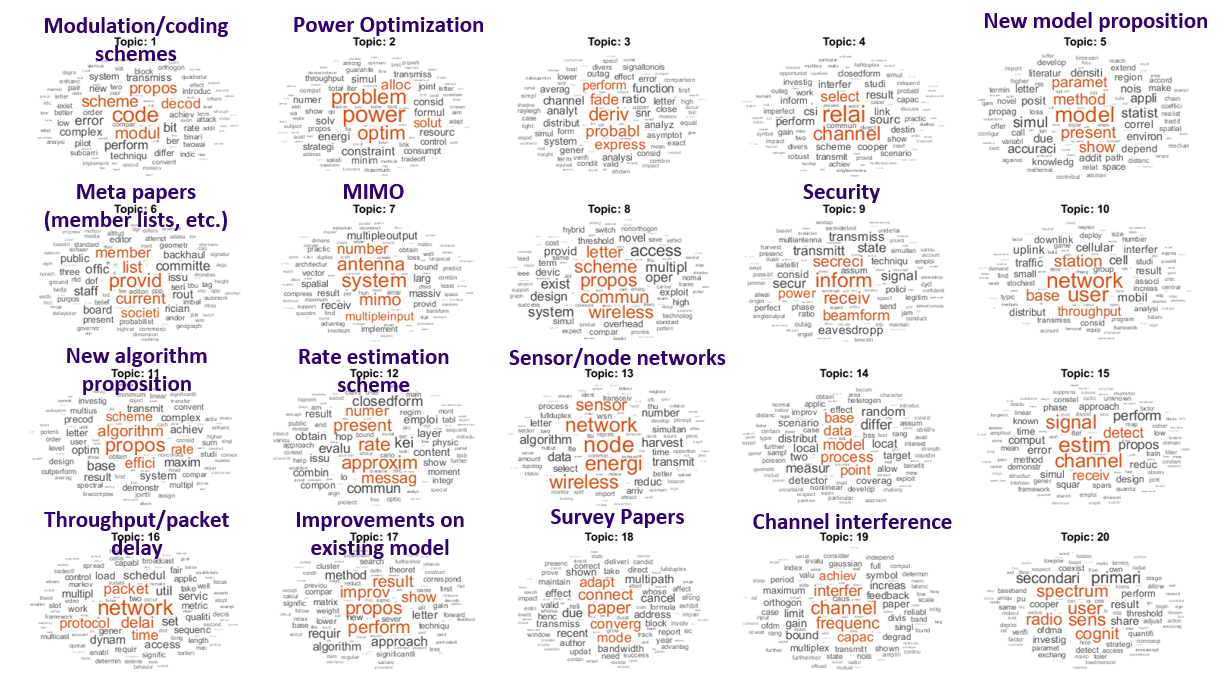
\includegraphics[width=3.49in]{wirelesscomm_topics.png}
	\caption{Annotated Topics in IEEE TRansactions on Wireless Communications}
	\label{fig:wirelesscomm_topics}
\end{figure}

\section{Conclusions}

The method presented here serves to prove that a comprehensive analysis of the body of academic work via the foremost natural language processing methodologies serves as an invaluable tool in a researcher's hands. The state of any academic field is ever-changing; a constant collection of fluid and yet dense documents that is difficult for anyone to keep up with. By making use of the tools presented here, a smart researcher can survey their field and get a feel for where their paper would be most well received, in additional for gaining knowledge about current trends and gaps in the body of knowledge.

By using an accessible and easily understood platform such as MATLAB, the resources here are outlined clearly for any research to make use of. A complete copy of the scripts used for processing can be found in the Appendix following, or on the author's personal Github at \url{https://github.com/stewythe1st/Research-Mining}.

\bibliographystyle{IEEEtran}
\bibliography{sources}

\end{document}